\documentclass[]{foi} 

\usepackage[utf8]{inputenc}
\usepackage{lipsum}

\vrstaRada{\projekt}

\title{Identificiranje korisnika pomoću dinamike tipkanja}
\predmet{\predmetSI}

\author{Karlo Vardijan, Lovro Pejaković, Filip Šoštarić, Stanko Smrček} 

\spolStudenta{\musko} 

\mentor{Bogdan Okreša Đurić}
\spolMentora{\musko} 
\titulaProfesora{dr. sc.}

\godina{2024}
\mjesec{ožujak}

\indeks{0016147086, 0016150223, 0016149647, 0016149535}

\smjer{Informacijsko i programsko inženjerstvo}


\sazetak{Opsega od 100 do 300 riječi. Sažetak upućuje na temu rada, ukratko se iznosi čime se rad bavi, teorijsko-metodološka polazišta, glavne teze i smjer rada te zaključci.}
% abstract of 100 to 300 words.

\kljucneRijeci{riječ; riječ; ...riječ; Obuhvaća $7\pm2$ ključna pojma koji su glavni predmet rasprave u radu.}
% keywords including 7 +/- 2 syntagms

\acrodef{VAS}{višeagentni sustav}



\begin{document}

\maketitle

\tableofcontents

\makeatletter \def\@dotsep{4.5} \makeatother
\pagestyle{plain}



\chapter{Uvod}

Cilj ovog projekta je analizom dinamike tipkanja identificirati korisnika. U ovom radu opisat će se sama dimanika tipkanja kao biometrijska karakteristika, u kojim područjima se primjenjuje i karakteristične mjere koje pohranjujemo te pomoću kojih na kraju vršimo samo identifikaciju. Biti će spomenuti sigurnosni rizici vezani za uporabu dinamike tipkanja i algoritmi strojnog učenja koji se koriste kod identifikacije. Detaljnije će se opisati metoda odabrana za praktični dio projekta. Na kraju slijedi opis implementiranog sustava za identifikaciju korisnika pomoću dinamike tipkanja.

\chapter{Dinamika tipkanja kao biometrijska karakteristika}
Identifikacija je proces određivanja identiteta osobe bez prethodne deklaracije od strane osobe koju pokušavamo identificirati.\cite{Kasprowski2022} Identifikacija se može smatrati kao 1 naprema više veza jer iz nekog skupa korisnika pokušavamo odrediti kome pripadaju karakteristike pomoću kojih vršimo sam proces identifikacije. Značajke koje se koriste u biometriji se dijele na fizičke i ponašajne. Fizičke uključuju stvari poput otiska prsta i strukture lica dok ponašajne obuhvaćaju način hoda, glas, potpis te dinamiku tipkanja.\cite{Kasprowski2022}

Za razliku od fizičkih karakteristika koje su unikatne od osobe do osobe, ponašajne karakteristike se mijenjaju tijekom vremena te nisu toliko pouzdane što se tiče sigurnosti. Ponašajne karakteristike su obično implementirane kao potpora fizičkim. Na ponašajne karakteristike utječu stvari poput emocionalnog stanja osobe, zdravstvenih uvjeta te uvjeta okoline. Gore navedene stvari su primjenjive na dinamiku tipkanja koja je fokus ovog projekta. Obje vrste karakteristika moraju ispunjavati uvjete koje biometrijske karakteristike trebaju imati. To su jedinstvnenost, univerzalnost, lakoća prikupljanja, nepromjenjivost i prihvatljivost.\cite{Kasprowski2022} Jedinstvenost kaže da bi karakteristika trebala biti jedinstvena za osobu tj. dvije osobe nebi smjele imati identičnu mjeru neke značajke. Univerzalnost znači da bi sve osobe morale posjedovati tu značajku. Značajka bi trebala biti lako prikupljiva te se nebi trebala mijenjati kroz vrijeme. Također mora biti korisničko prihvatljiva. Prvi primjeri korištenja dinamike tipkanja u svrhu identifikacije pojavili su se tijekom 2. Svjetskog Rata kod slanja poruka Morsovim kodom. Način na koji je poruka otipkana mogla je dati uvid u legitimnost poruke.\cite{Haring2007}

Postojeća rješenja i implementacije bazirane su na statističkim podacima određenih događaja. Događaji koji se uglavnom koriste su duljine trajanja između pritiska i odpuštanja jedne tipke (eng. Dwell time), vrijeme koje protekne između odpuštanja jedne te pritiska druge tipke (eng. Interval), vrijeme između otpuštanja prve te odpuštanja druge tipke (eng. Up to up), vrijeme između pritiska prve tipke te pritiska druge (eng. Flight time), vrijeme između pritiska prve tipke te odpuštanja druge scenariji u kojima se koriste "Shift" i "Capslock" tipke za pisanje velikih slova i korištenje strelica za pozicioniranje u tekstu.\cite{Kasprowski2022} Manje korištene značajke uključuju i poziciju prsta na tipkama što zahtjeva korištenje kamere. Također se može promatrati i odabir prstiju koji se koristi za određene tipke za koje je također potrebna kamera.
Kod procesa identifikacije koriste se dvije vrste tekstova: oni s definiranim brojem znakova i oni s nasumično odabranom duljinom.\cite{Kasprowski2022} Podaci o dinamici tipkanja se obično prikupljaju tipkovnicom, no kako su pametni mobiteli u današnje vrijeme sveprisutni, moguće je i na taj način obaviti prikupljanje. Ovdje također možemo zabilježiti točne koordinate pritiska, veličinu ekrana koju prst prekriva kod određene tipke te jačinu pritiska.\cite{Lee2018}

\chapter{Skup podataka dinamičkog tipkanja}
Za ovaj rad pronašli smo besplatni skup podataka za dinamičko tipkanje KeyRecs. Skup podataka je dobiven od 99 sudionika koji su sudjelovali u dva zadatka  \cite{Dias2023}. Prvi zadatak je bio pisanje lozinke „vpwjkeurkb“ 200 puta kroz dvije sesija, a drugi zadatak je bio prepisivanje 10 odlomaka raznih literatura isto kroz dvije sesije \cite{Dias2023}. Ti zadaci su se provodili preko web stranice koja je bilježila razna vremena tijekom tipkanja \cite{Dias2023}. Vremena koja su se bilježila su: od pritiska tipke do puštanja tipke (DU), od pritiska tipke do pritiska druge tipke (DD), od puštanja tipke do pritiska druge tipke (UD), od puštanja tipke do puštanja druge tipke(UU), od pritiska tipke do puštanja druge tipke (DU) i ukupno vrijeme tipkanja \cite{Dias2023}. Ta vremena su dobro prikazana na slici \ref{fig:graf-vremena-tipkanja}. Osim tih vremena za svakoga korisnika su  zabilježene: godine, spol, nacionalnost i dominantna ruka  \cite{Dias2023}. Podaci za prvi zadatak pisanja lozinke su zapisani kao tablica \ref{tab:KeyRecs-podaci}. U svakom redu je zabilježeno: tko je pisao, koja je sesija, koje ponavljanje i vremena za svaku tipku sifre \cite{Dias2023}. Vremena su zabilježena u kolone (D|U).tipka1.tipka2 gdje prvi dio prikazuje određeno vrijeme na temelju slike \ref{fig:graf-vremena-tipkanja} a druga dva dijela na koju tipku se odnosi \cite{Dias2023}.

\begin{table}[!h]
    \centering
    \caption{Dio podataka iz KeyRecs skupa podataka; prema \cite{Dias2023}}
    \begin{tabularx}{1\textwidth}{|l|l|l|l|l|l|l|l|l|l|}
    \hline
        \cellcolor{gray!25}participant & \cellcolor{gray!25}session & \cellcolor{gray!25}repetition & \cellcolor{gray!25}DU.v.v & \cellcolor{gray!25}DD.v.p & \cellcolor{gray!25}DU.v.p & \cellcolor{gray!25}UD.v.p & \cellcolor{gray!25}UU.v.p & \cellcolor{gray!25}DU.p.p & \cellcolor{gray!25}... \\ \hline
        p001 & 1 & 1 & 0.129 & 1.917 & 1.804 & 2.046 & 1.933 & 0.113 & ... \\ \hline
        p001 & 1 & 2 & 0.112 & 0.192 & 0.096 & 0.304 & 0.208 & 0.096 & ... \\ \hline
        p001 & 1 & 3 & 0.088 & 0.253 & 0.182 & 0.341 & 0.27 & 0.071 & ... \\ \hline
        ... & ... & ... & ... & ... & ... & ... & ... & ... & ... \\ \hline
    \end{tabularx}
    \\[10pt]
    \label{tab:KeyRecs-podaci}
\end{table}


\begin{figure}[!h]
    \centering
    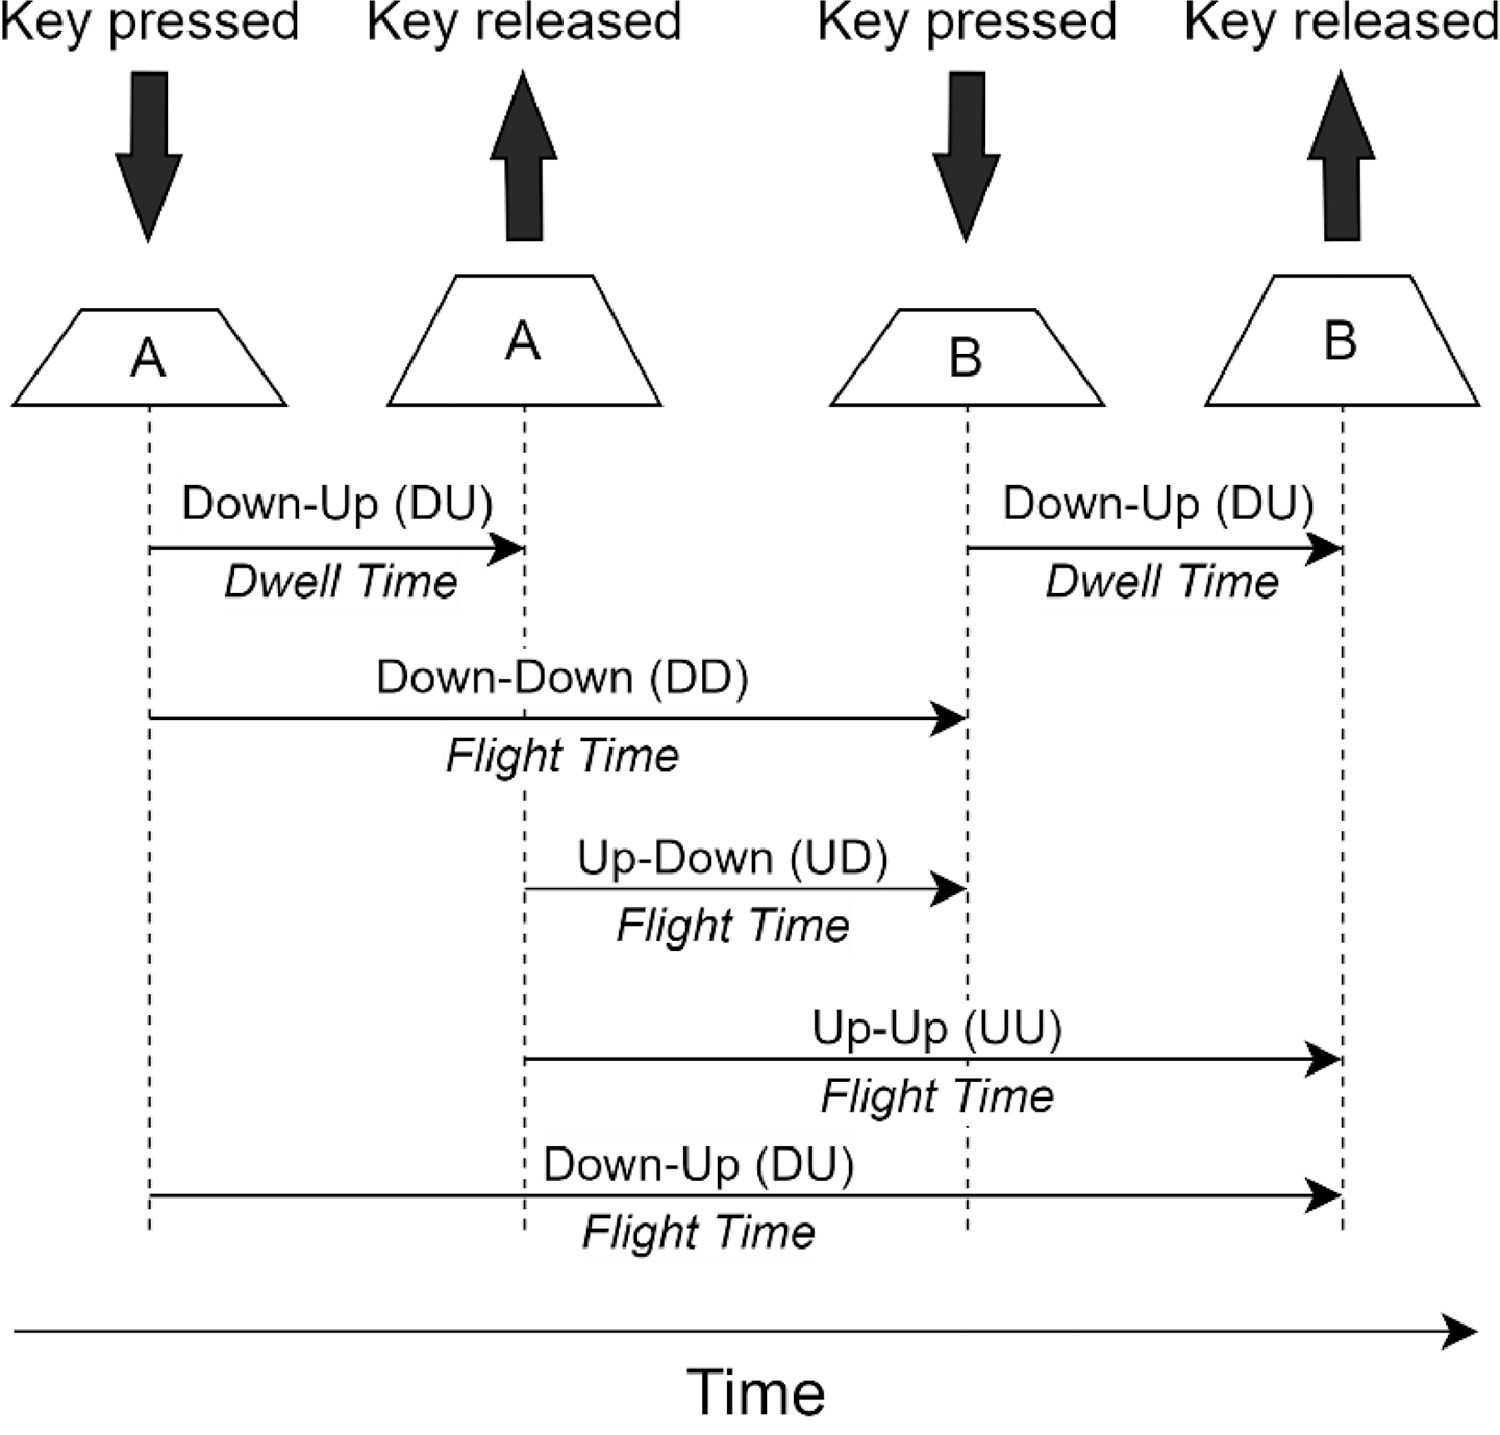
\includegraphics[width=0.6\textwidth]{slike/tipkanje-graf.jpg}
    \caption{Grafikon bilježenih vremena tijekom tipkanja; preuzeto iz \cite{Dias2023}}
    \label{fig:graf-vremena-tipkanja}
\end{figure}


\chapter{Metode analize dinamike tipkanja pomoću umjetne inteligencije}




\chapter{IZBRISI POSLIJE}

Ovo je glavni dio rada u kojem treba razraditi temu, pojasniti istraživanja, prikazati rezultate i slično. Poželjno je na početku poglavlja dati kratki opis strukture poglavlja, kako bi čitatelj/čitateljica rada mogao/mogla lakše pratiti složenu cjelinu.



\section{Poglavlje druge razine }

\lipsum[6]



\subsection{Poglavlje treće razine}

\lipsum[2]



\subsection{Poglavlje četvrte razine}

\lipsum[4-5]



\chapter{IZBRISI POSLIJE}

Tehničke upute u nastavku opisuju način tehničkog oblikovanja rada i navođenja literature.



\section{Upute za oblikovanje izgleda rada}

\subsection{Oblikovanje stranice}

\textbf{Stranice} su oblikovane korištenjem sljedećih parametara:

\begin{itemize}
    \item veličina i oblik papira je A4, okomito usmjerenje, margine 2,5 cm na svakoj strani;

    \item naslovna stranica rada se ne numerira;

    \item nakon naslovne stranice, sve sljedeće stranice do 1. Poglavlja se numeriraju rimskim brojevima, počevši od i;

    \item od 1. poglavlja nadalje, stranice se numeriraju arapskim brojevima;

    \item broj stranice treba pozicionirati desno 1,25 cm od dna stranice, font Arial 9.
\end{itemize}

\subsection{Tekst rada}

\textbf{Tekst} rada je oblikovan na sljedeći način:
\begin{itemize}
    \item u pisanju teksta koristite font Arial 11 pt, s proredom 1,5 te razmakom 0 pt prije i razmakom 6 pt poslije odlomka, pri čemu je prvi redak uvučen za 1,25 cm;

    \item u naslovima prve razine „3. Razrada teme“ koristite font Arial 18 pt, podebljano, prijelom stranice (svaki naslov prve razine treba biti na novoj stranici), s proredom 1,5 te razmakom 0 pt prije i razmakom 18 pt poslije odlomka;

    \item u naslovima druge razine „2.1. Naslov“ koristite font Arial 16 pt, podebljano, s proredom 1,5 te razmakom 18 pt prije i razmakom 12 pt poslije odlomka;

    \item u naslovima treće razine „2.1.1. Naslov“ koristite font Arial 14 pt, podebljano, s proredom 1,5 te razmakom 12 pt prije i razmakom 6 pt poslije odlomka;

    \item u naslovima četvrte razine „2.1.1.1. Naslov“ koristite font Arial 12 pt, podebljano, s proredom 1,5 te razmakom 6 pt prije i razmakom 6 pt poslije odlomka;

    \item ostalo značajno isticanje cjelina rada može biti istaknuto podebljanim i kurziv slovima, korištenjem fonta Arial 11 pt.
\end{itemize}

\subsection{Slike}

\textbf{Slike} u radu je potrebno oblikovati na sljedeći način:

\begin{itemize}
    \item opis slike navedite ispod slike uz numeraciju;
    
    \item za nazive slika koristite iste postavke fonta kao i za tekst, ali stavite opis slike u centrirani položaj;

    \item za oblikovanje same slike koristite font Arial 9 pt za tekst na slici;
ispred same slike umetnite jedan prazan redak (osim ako je slika pozicionirana na početku stranice);

    \item kod prijeloma stranice treba obratiti posebnu pozornost da opis slike, izvor i sama slika moraju biti na istoj stranici; 

    \item slike je potrebno numerirati redom pojavljivanja u tekstu;

    \item ako je slika preuzeta iz drugog izvora, nakon navođenja opisa slike je potrebno dodati i referencu izvornog djela;

    \item dozvoljeno je napraviti vlastitu preradu slika, grafikona ili tablica na način da se zadrži isti smisao sadržaja, ali promijeni izgled, pri čemu je obavezno u opisu slike navesti referencu izvornog djela ovako: <opis slike> ; prema [X]

    \item dozvoljeno je preuzeti samo jednu sliku, grafikon ili tablicu u izvornom obliku iz istog izvora. Za doslovno preuzimanje većeg dijela sadržaja potrebno je ishoditi dozvolu nositelja autorskih prava;

\end{itemize}


\subsection{Tablice}

\textbf{Tablice} rada je potrebno oblikovati sukladno ovim uputama:
\begin{itemize}
    \item opis tablice navedite iznad slike;

    \item za opise tablica koristite iste postavke fonta kao i za tekst, ali stavite opis tablice u centrirani položaj;

    \item za oblikovanje same tablice koristite font Arial 9 pt za tekst u tablici;

    \item tablice numerirajte redom pojavljivanja u tekstu;

    \item kod prijeloma stranice treba obratiti posebnu pozornost da opis tablice, izvor i sama tablica moraju biti na istoj stranici; 

    \item ako je tablica preuzeta iz drugog izvora, nakon navođenja opisa tablice potrebno je navesti izvor, na isti način kako je opisano kod slika;

    \item primjer označavanja tablice možete vidjeti u nastavku (tablica \ref{tab:objekti}).
\end{itemize}

\begin{table}[h!] 
    \centering
    \caption{Prikaz podataka o učestalosti pojavljivanja objekta; prema \cite{wooldridge2009IntroductionMultiAgentSystems}}
    \begin{tabularx}{0.66\textwidth}{|X|X|X|X|}
        \hline
         \cellcolor{gray!25} & \cellcolor{gray!25} & \cellcolor{gray!25} & \cellcolor{gray!25} \\
        \hline
         &  &  &  \\
        \hline
         &  &  & \\
        \hline
    \end{tabularx}
    \\[10pt]
    \label{tab:objekti}
\end{table}

\subsection{Programski kod}

Za oblikovanje teksta koji je programski kod korišten je font Courier, veličine 10 pt, jednostruki prored, 6 pt iza odlomka, npr. HTML kod dijela zaglavlja početne web stranice FOI weba je prikazan kao isječak koda \ref{lst:dva}.

\begin{listing}
    \begin{minted}{xml}
<head>
  <meta http-equiv="Content-Type" content="text/html; charset=utf-8" />
  <link rel="shortcut icon" href="https://www.foi.unizg.hr/sites/default/files/favicon_0_1.ico" type="image/vnd.microsoft.icon" />
  <meta name="generator" content="Drupal 7 (http://drupal.org)" />
  <link rel="canonical" href="https://www.foi.unizg.hr/hr" />
  <link rel="shortlink" href="https://www.foi.unizg.hr/hr" />
  <!-- Set the viewport width to device width for mobile -->
  <meta name="viewport" content="width=device-width, initial-scale=1.0">
  <title>Dobro %*došli*) na FOI | FOI</title>...
</head>
    \end{minted}
    \caption{Primjer isječka koda}
    \label{lst:dva}
\end{listing}

U slučaju preuzetog programskog koda, za isti je nužno potrebno naznačiti izvor, kao u isječku koda \ref{lst:kod2}. 

Ponekad palatali mogu stvarati probleme u opisima isječaka koda, pa ih je potrebno zamijeniti \LaTeX\ kodovima: \v{c}/\v{s}/\v{z}: \mintinline{text}{\v{c/s/z}}, \'{c}: \mintinline{text}{\'{c}}, \dj: \mintinline{text}{\dj}.


\begin{listing}
    \begin{minted}{python}
print("Ovo je preuzeti dio koda")
    \end{minted}
    \caption[Ovo je primjer koda koji je preuzet]{Ovo je primjer koda koji je preuzet iz \cite[str. 23]{russell2022ArtificialIntelligenceModern}}
    \label{lst:kod2}
\end{listing}



\subsection{Formule}

Za unos formula koristite editor za formule. Matematičke izraze moguće je pisati unutar teksta $E = mc^2$ ili izdvojeno:
    
$$
a^2 + b^2 = c^2
$$

\subsection{Kratice}

Želite li koristiti kratice pojmova u tekstu, kad prvi put spominjete pojam potrebno je navesti puni naziv, a kraticu navesti u zagradi: informacijske i komunikacijske tehnologije (IKT). Nakon toga možete koristiti kratice u tekstu. Poželjno je u naslovima koristiti pune nazive.

Kratice je moguće definirati i korištenjem naredbe \mintinline{text}{\acrodef{}{}}, iz \mintinline{text}{acronym} paketa, prije početka dokumenta (naredba \mintinline{text}{\begin{document}}). Tako definirane kratice pozivaju se unutar dokumenta naredbom \mintinline{text}{\ac{}} ili \mintinline{text}{\Ac{}} za veliko početno slovo. 

\subsection{Strano nazivlje}

Strano nazivlje se u tekstu navodi u zagradi, napisano \textit{kurzivom}, nakon hrvatskog izraza, npr. analiza društvene mreže (engl. \textit{Social Network Analysis - SNA}).



\section{Navođenje literature}

Za navođenje literature u radu koristite \textbf{IEEE} stil. Važno je dosljedno primjenjivati odabrani stil u cijelom radu.

U popisu literature potrebno je navesti svu literaturu i samo literaturu koju ste koristili u tekstu.

Uz svaku preuzetu tvrdnju potrebno je navesti njezin izvor, tj. referencu. Reference se u tekstu navode tako da se uz citirani tekst navede izvor, sukladno načinu propisanom odabranim stilom i FOI preporukama za citiranje i referenciranje \cite{sveucilisteuzagrebufakultetorganizacijeiinformatike2017FOIPreporukeCitiranja}. Prilikom referenciranja knjiga, uvijek je potrebno navoditi i broj ili brojeve stranica.

Za citate i njihovo referenciranje koristite naredbu \mintinline{text}{\blockquote} kako slijedi. Citat će se automatski oblikovati kako je potrebno, ovisno o duljini citata. U kratkom citatu je pojašnjeno da bi se hibridna platforma za orkestraciju mogla u domeni videoigara koristiti
\blockquote[{\cite[str. 5]{schatten2020PlatformeZaOrkestraciju}}]{za implementaciju većeg broja inteligentnijih, a samim
time i interesantnijih, suparnika.} Ono što slijedi nakon obavezno navedenog broja stranice uz izvor citata je primjer duljeg citata.

\blockquote[{\cite[str. 6]{schatten2020PlatformeZaOrkestraciju}}]{Iako je testiranje performansi MMO igara dobro implementirano na brojnim platformama, testiranje iskustva
igranja (posebno u primjerice MMORPG igrama) velikog razmjera postaje iznimno složen zadatak, kao što
je okvirno predstavljeno u (Schatten, Okreša Ðurić, Tomičić i Ivković, 2017). Ne samo da je potrebno testirati
razne logičke zagonetke i zadatke koje igrač mora riješiti kako bi napredovao u igri, već i pojavljujuću interakciju među igračima koja bi mogla u potpunosti promijeniti rezultat igre. Korištenjem distribuirane platforme za orkestraciju bilo bi moguće dodavanje automatiziranih igrača po volji instanciranjem novih agenata. Štoviše, rezultati testiranja mogli bit biti dodatno
analizirani dodavanjem agenata za analizu ili izvještavanje.}

Podaci o svim bibliografskim jedinicama nalaze se u \mintinline{text}{lib.bib} datoteci u \mintinline{text}{BibLaTeX} formatu. Bibliografske jedinice korištene u ovom dokumentu su:
\begin{itemize}
    \item knjige \cite{russell2022ArtificialIntelligenceModern,wooldridge2009IntroductionMultiAgentSystems,oraictolic2011AkademskoPismoStrategije},
    \item članak s konferencije \cite{okresaduric2019ModellingFormingTemporary},
    \item članci iz časopisa \cite{SchattenEtAl2016roadmap,rincon2017InfluencingPeopleSocial},
    \item web-stranica \cite{copeland2020ArtificialIntelligence}.
\end{itemize}






\chapter{Zaključak - napiši}

Ovdje treba sažeto rezimirati najvažnije rezultate razrade teme rada. Potrebno je sažeto opisati što je predmet rada \cite{copeland2020ArtificialIntelligence}, koje su metode, tehnike, programski alati ili aplikacije korištene u razradi rada te koje su pretpostavke dokazane, a koje opovrgnute. Sadržajno, ono što se u uvodu rada najavljuje i kasnije je obuhvaćeno u samom radu, moralo bi biti opisano u zaključnom dijelu kroz rezultate rada. \cite{Kasprowski2022}


\makebackmatter

\end{document}
